% modified from NeurIPS 2022 Latex template
% authors: Yixin Zhu (yixin.zhu@pku.edu.cn), Liangru Xiang
% v1.0: 2022.07.21

\documentclass{article}
\PassOptionsToPackage{numbers,compress}{natbib}
\usepackage[final]{template22}
\input{config.tex}

\title{Humanoid Parkour Locomotion for Unitree G1 in Isaac Lab}
\newcommand{\runningauthor}{Mao RuoLin}
\newcommand{\runningid}{2026-AI-Practice}

\author{%
  Mao RuoLin \\
  Yuanpei College \\
  Peking University \\
  \texttt{2400017736@stu.pku.edu.cn} \\
}

\begin{document}
\maketitle

\begin{abstract}
Robust humanoid locomotion over structured obstacles remains difficult because a policy must simultaneously track commands, maintain balance, and handle terrain discontinuities such as stairs, boxes, slopes, and gaps. This project builds a custom parkour-oriented locomotion task for the Unitree G1 robot in Isaac Lab. Starting from the official manager-based G1 rough locomotion task, I implement three increasing parkour terrain tiers, train PPO policies with RSL-RL, and evaluate them with survival, traversal-progress, and geometry-aware obstacle-crossing metrics. The results show a clear terrain difficulty gradient: easy parkour is stable, medium parkour is the first tier that transfers strongly to hard terrain, and hard parkour is the strongest source policy, reaching at least 95.31\% timeout rate across rough/easy/medium/hard evaluation environments and 100.00\% hard gap/stairs obstacle pass rate under the fixed-row stress protocol. A reward-shaping MDP ablation further shows that adding parkour-progress and foothold-safety terms to rough-terrain training improves hard-terrain timeout rate from 29.69\% to 70.31\% without any parkour terrain exposure. On hard terrain, the foothold-safety term mainly improves tracking precision and medium-gap crossing at the cost of lower forward speed. An additional ExtremeRandom out-of-distribution stress test confirms the same safety-vs-speed pattern. Overall, the project delivers a reproducible parkour task package, training scripts, evaluation pipeline, and quantitative analysis for humanoid obstacle locomotion.
\end{abstract}

\section{Introduction}
\label{sec:introduction}

Humanoid parkour locomotion requires more than stable flat-ground walking. A useful policy must move over uneven terrain, climb or descend structured height changes, cross gaps, and avoid falls while still obeying a locomotion command. The goal of this project is to build a reproducible parkour-oriented locomotion environment for the Unitree G1 robot in Isaac Lab. The project extends an existing locomotion task with custom terrain design, reinforcement-learning training, systematic evaluation, and ablation analysis.

The repository is a compact Isaac Lab task package. It stores task registration code, terrain configurations, reward extensions, scripts and results. Isaac Lab itself remains an external dependency. Large artifacts such as checkpoints and TensorBoard event files are kept outside the repository.

The project repository is available at: \url{https://github.com/shenshan222/g1-parkour-isaaclab}.

The main contributions are:
\begin{itemize}[leftmargin=*,noitemsep,nolistsep,topsep=0pt]
    \item three custom parkour terrain tiers for Unitree G1, covering stairs, boxes, rough patches, slopes, and gaps;
    \item a training and play pipeline for easy, medium, and hard parkour tasks using PPO through RSL-RL;
    \item a unified evaluation pipeline with timeout, traversal-progress, and obstacle-crossing metrics;
    \item a terrain difficulty ablation across flat, rough, easy, medium, and hard settings;
    \item a reward-shaping MDP ablation using parkour-progress and foothold-safety rewards;
    \item an additional ExtremeRandom out-of-distribution stress evaluation for hard and hard-MDP policies.
\end{itemize}


\section{Method}
\label{sec:method}

\subsection{Framework and task objective}

The task is built on Isaac Lab's manager-based Unitree G1 rough velocity-tracking environment. The inherited environment provides the robot model, low-level actuation interface, proprioceptive observations, height-scan sensing, terrain curriculum machinery, and base-contact failure termination. This project keeps the underlying locomotion interface unchanged and studies how terrain curriculum, reward shaping, and evaluation metrics affect obstacle locomotion.

At each episode, the policy is commanded to track a planar velocity command while moving over a generated terrain tile. A successful parkour policy should therefore satisfy three requirements at the same time: it should avoid falling, maintain reasonable command tracking, and make forward progress across terrain discontinuities such as stairs and gaps.

\subsection{MDP formulation}

I model the task as a finite-horizon Markov decision process
\begin{equation}
    \mathcal{M} = (\mathcal{S}, \mathcal{A}, p, r, \gamma, T).
\end{equation}
The state $s_t$ is represented through Isaac Lab manager terms, including base and joint states, projected gravity, commanded velocity, previous action, contact information, and terrain height-scan observations. The action $a_t$ is a vector of joint-position targets for the G1 robot. The transition $p(s_{t+1}\mid s_t,a_t)$ is induced by Isaac Sim physics, terrain geometry, contact dynamics, and the command sampler.

The inherited G1 rough task already contains the base velocity-tracking, posture, action regularization, and failure-related reward terms. Parkour training adds a forward-progress reward:
\begin{equation}
    r_t = r_t^{\mathrm{G1}} + w_p r_t^{\mathrm{progress}},
    \qquad
    r_t^{\mathrm{progress}} = \mathrm{clip}(0.5 v_{x,t}^{w}, 0, 0.75),
    \qquad
    w_p = 0.5,
\end{equation}
where $v_{x,t}^{w}$ is the base velocity along the world $x$ axis. This term is deliberately simple: it does not identify individual obstacles, but it biases the policy toward traversing the terrain rather than only surviving in place.

The MDP ablation adds a foothold-safety cost while keeping the robot, observations, action space, terrain generator, PPO algorithm, and evaluation protocol fixed:
\begin{equation}
    r_t^{\mathrm{MDP}} =
    r_t^{\mathrm{G1}} + w_p r_t^{\mathrm{progress}} - w_f c_t^{\mathrm{foothold}},
    \qquad
    w_f = 0.2.
\end{equation}
The cost is
\begin{equation}
    c_t^{\mathrm{foothold}} =
    c_t^{\mathrm{slide}} + 2.0 c_t^{\mathrm{drop}} + 0.5 c_t^{\mathrm{mismatch}}.
\end{equation}
Here $c_t^{\mathrm{slide}}$ penalizes foot sliding while a foot is in contact, $c_t^{\mathrm{drop}}$ penalizes support points that drop far below the base as a proxy for edge or gap stepping, and $c_t^{\mathrm{mismatch}}$ penalizes large height differences between simultaneously contacting feet. A stricter early fall termination was tested during development but removed from the final MDP because it ended episodes too early and prevented exploration. The final tasks use the inherited base-contact termination.

\subsection{Parkour terrain curriculum}

The parkour curriculum replaces the official rough terrain generator with three terrain presets. Each preset mixes structured terrain components such as stairs, boxes, rough patches, slopes, and, for medium and hard tiers, gaps. The key difficulty ranges are summarized in \Cref{tab:terrain-curriculum}.

\begin{table}[t]
    \caption{\textbf{Parkour terrain curriculum.} Difficulty increases through higher steps and boxes, wider gaps, stronger slopes, and narrower feasible platforms.}
    \label{tab:terrain-curriculum}
    \centering
    \begin{tabular}{lccc}
        \toprule
        Terrain parameter & Easy & Medium & Hard \\
        \midrule
        Step height & 0.05--0.17 m & 0.05--0.23 m & 0.10--0.28 m \\
        Gap width & none & 0.05--0.28 m & 0.15--0.45 m \\
        Box/grid height & 0.05--0.15 m & 0.05--0.20 m & 0.08--0.25 m \\
        Slope range & up to 0.30 & up to 0.40 & up to 0.45 \\
        \bottomrule
    \end{tabular}
\end{table}

\subsection{Evaluation metrics}

The evaluation pipeline reports three success criteria. Timeout success means an episode reaches the horizon without base-contact failure. Traversal-progress success means the robot avoids failure and reaches at least 4 m forward displacement. Obstacle-crossing success means the robot avoids failure and its base crosses the generated geometry boundary of a supported gap or stairs obstacle. Timeout measures survival, progress distinguishes survival from standing still, and obstacle crossing measures terrain-specific completion.

\section{Experimental setup}
\label{sec:setup}

All completed training runs were executed on an AutoDL Linux GPU environment with an NVIDIA GeForce RTX 3090. Isaac Lab was installed externally, while this repository was installed as an editable task package. Policies were trained with PPO through RSL-RL using the inherited G1 rough runner configuration unless otherwise stated. 

\Cref{tab:runs} summarizes the training runs used throughout this report. The table separates official Isaac Lab baselines, custom parkour terrain policies, and reward-shaping MDP variants. 

\begin{table}[t]
    \caption{\textbf{Training runs.} All parkour and MDP policies are trained for 3000 PPO iterations.}
    \label{tab:runs}
    \centering
    \begin{tabular}{llc}
        \toprule
        Experiment & Task family & Iterations \\
        \midrule
        Flat baseline & official flat G1 & 1500 \\
        Rough baseline & official rough G1 & 3000 \\
        Parkour easy & custom easy parkour & 3000 \\
        Parkour medium & custom medium parkour & 3000 \\
        Parkour hard & custom hard parkour & 3000 \\
        Rough MDP & rough terrain with MDP rewards & 3000 \\
        Hard MDP & hard parkour with MDP rewards & 3000 \\
        \bottomrule
    \end{tabular}
\end{table}

The official flat baseline uses \texttt{Isaac-Velocity-Flat-G1-v0}. The rough baseline uses \texttt{Isaac-Velocity-Rough-G1-v0} and is the direct parent of all parkour tasks. The three parkour training tasks are \texttt{Isaac-Velocity-Parkour-G1-Easy-v0}, \texttt{Isaac-Velocity-Parkour-G1-Medium-v0}, and \texttt{Isaac-Velocity-Parkour-G1-Hard-v0}; each has a corresponding play task for visualization and evaluation. The MDP variants are \texttt{Isaac-Velocity-Rough-G1-MDP-v0} and \texttt{Isaac-Velocity-Parkour-G1-Hard-MDP-v0}. Implementation files are concentrated in the environment configuration, terrain configuration, MDP override, and evaluation modules of the task package.

For cross-terrain evaluation, I load each source checkpoint and evaluate it on rough, easy, medium, and hard play environments. Random cross-terrain evaluation samples terrain type and difficulty inside the terrain grid, while fixed-row stress evaluation pins all environments to the highest difficulty row. Unless otherwise noted, cross/stress evaluations use 64 episodes, 32 parallel environments, and seed 42.

\section{Results}
\label{sec:results}

\subsection{Reference baselines}

\Cref{tab:baseline} compares the two official G1 baselines used to validate the project pipeline. The flat baseline verifies the training pipeline: it reaches 99.56\% timeout rate and only 0.44\% base-contact failure. The rough baseline is harder but remains stable, with 94.62\% timeout rate and 5.41\% base-contact failure. Its XY velocity tracking error is higher than the flat baseline, increasing from 0.2087 m/s to 0.3407 m/s. This confirms that the official rough task is a meaningful stepping stone between flat walking and parkour.


\begin{table}[t]
    \caption{\textbf{Baseline comparison.} Rough terrain increases failure rate and tracking error while preserving stable training.}
    \label{tab:baseline}
    \centering
    \begin{tabular}{lcc}
        \toprule
        Metric & Flat & Rough \\
        \midrule
        Mean reward & 28.77 & 24.01 \\
        Mean episode length & 1000.0 & 984.5 \\
        Timeout rate & 99.56\% & 94.62\% \\
        Base-contact failure & 0.44\% & 5.41\% \\
        XY tracking error & 0.2087 m/s & 0.3407 m/s \\
        \bottomrule
    \end{tabular}
\end{table}

\subsection{Parkour training}

\begin{figure}[t]
    \centering
    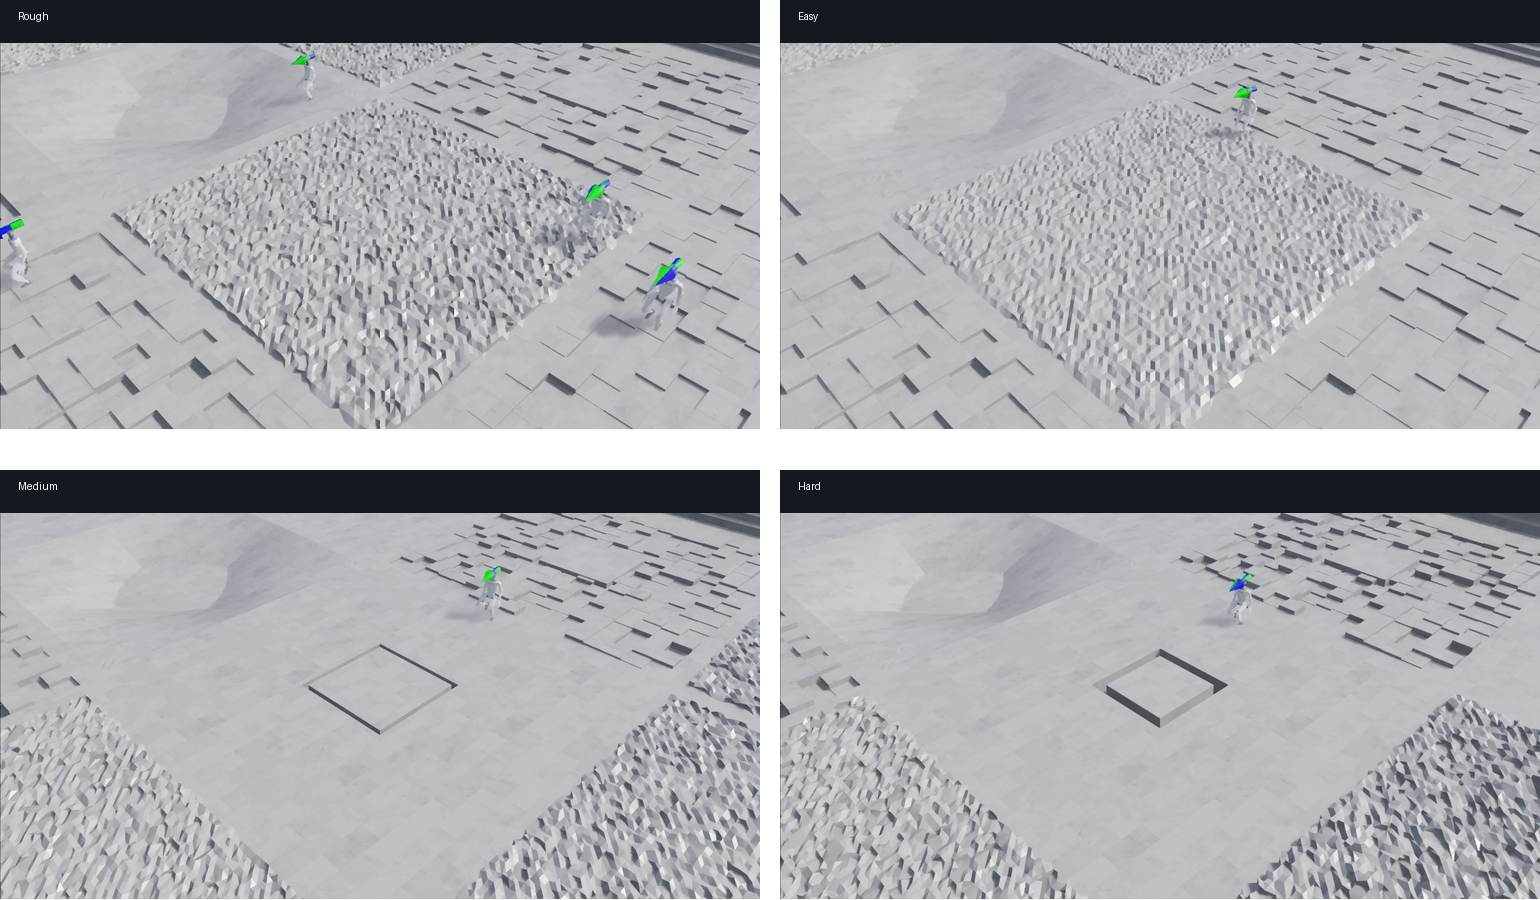
\includegraphics[width=0.96\linewidth]{figures/terrain_rollout_montage.png}
    \caption{\textbf{Policy rollouts on representative terrains.} Frames are extracted from the recorded rough, easy, medium, and hard play videos. They provide qualitative evidence that the learned policies are evaluated on visibly different terrain structures rather than on a single flat locomotion setting.}
    \label{fig:terrain-rollout}
\end{figure}

\Cref{fig:terrain-rollout} shows representative policy rollouts on rough and parkour terrains. The visual progression matches the quantitative curriculum: easy terrain mainly tests structured uneven walking, medium introduces gaps and stronger obstacles, and hard combines wider discontinuities with tighter feasible footholds.

\begin{table}[t]
    \caption{\textbf{Final training summary for parkour tiers.} The same 3000-iteration budget produces a clear difficulty gradient.}
    \label{tab:parkour-training}
    \centering
    \begin{tabular}{lccc}
        \toprule
        Metric & Easy & Medium & Hard \\
        \midrule
        Mean reward & 30.70 & 20.98 & 11.34 \\
        Mean episode length & 983.2 & 988.1 & 941.7 \\
        Timeout rate & 96.00\% & 93.25\% & 89.08\% \\
        Fall rate & 4.00\% & 6.75\% & 10.92\% \\
        XY tracking error & 0.3050 & 0.3590 & 0.4407 \\
        Yaw tracking error & 0.6067 & 0.8445 & 1.0088 \\
        Curriculum level & 5.7907 & 5.8001 & 5.6389 \\
        \bottomrule
    \end{tabular}
\end{table}

\Cref{tab:parkour-training} shows the expected terrain difficulty ordering. Easy parkour remains highly stable, medium parkour introduces a moderate degradation, and hard parkour has the lowest reward, highest fall rate, and largest velocity tracking error. The curriculum scalar is useful within each terrain preset but should not be interpreted as the same absolute physical difficulty across different terrain generators.


\subsection{Cross-terrain generalization}

The 4-by-4 cross-terrain evaluation loads rough/easy/medium/hard checkpoints and evaluates each on rough/easy/medium/hard play environments. Random cross-terrain evaluation samples terrain type and difficulty inside the terrain grid, while fixed-row stress evaluation uses the highest difficulty row for each terrain preset. I report three metrics: timeout rate, traversal-progress rate, and geometry-aware obstacle-crossing rate.

\begin{figure}[t]
    \centering
    \begin{subfigure}[t]{0.32\linewidth}
        \centering
        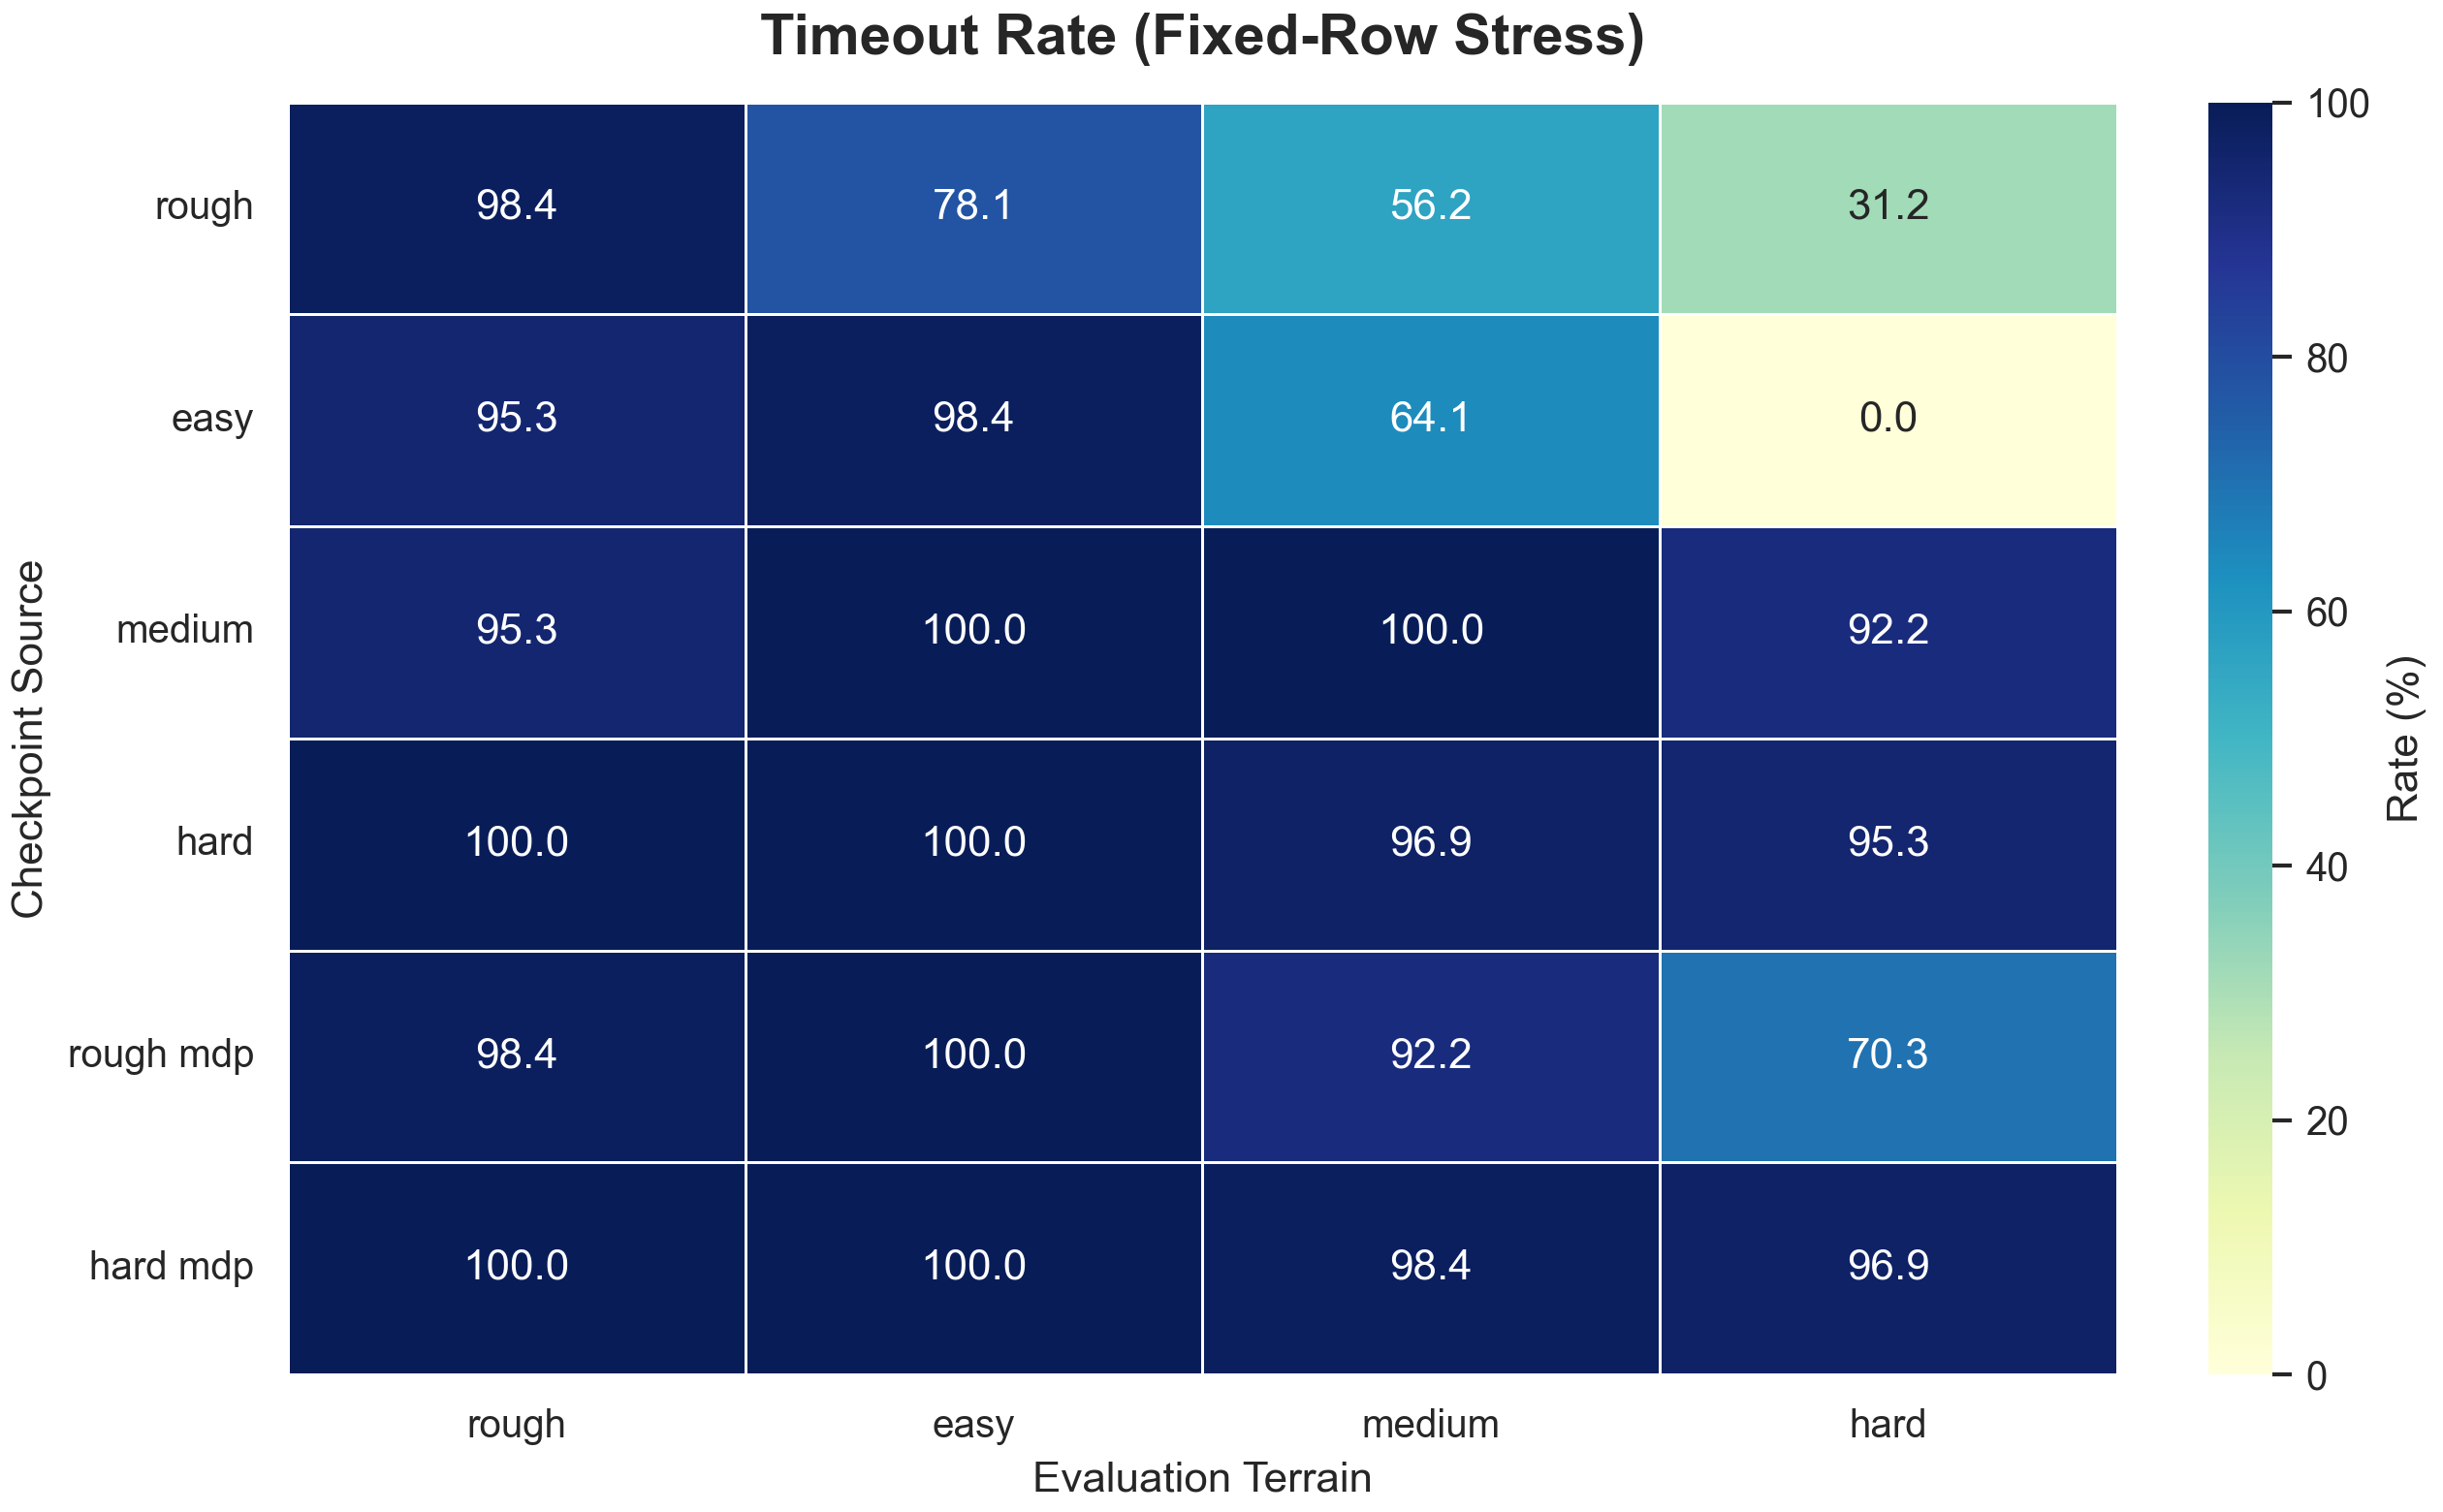
\includegraphics[width=\linewidth]{figures/timeout_stress_heatmap.png}
        \caption{Timeout}
    \end{subfigure}
    \hfill
    \begin{subfigure}[t]{0.32\linewidth}
        \centering
        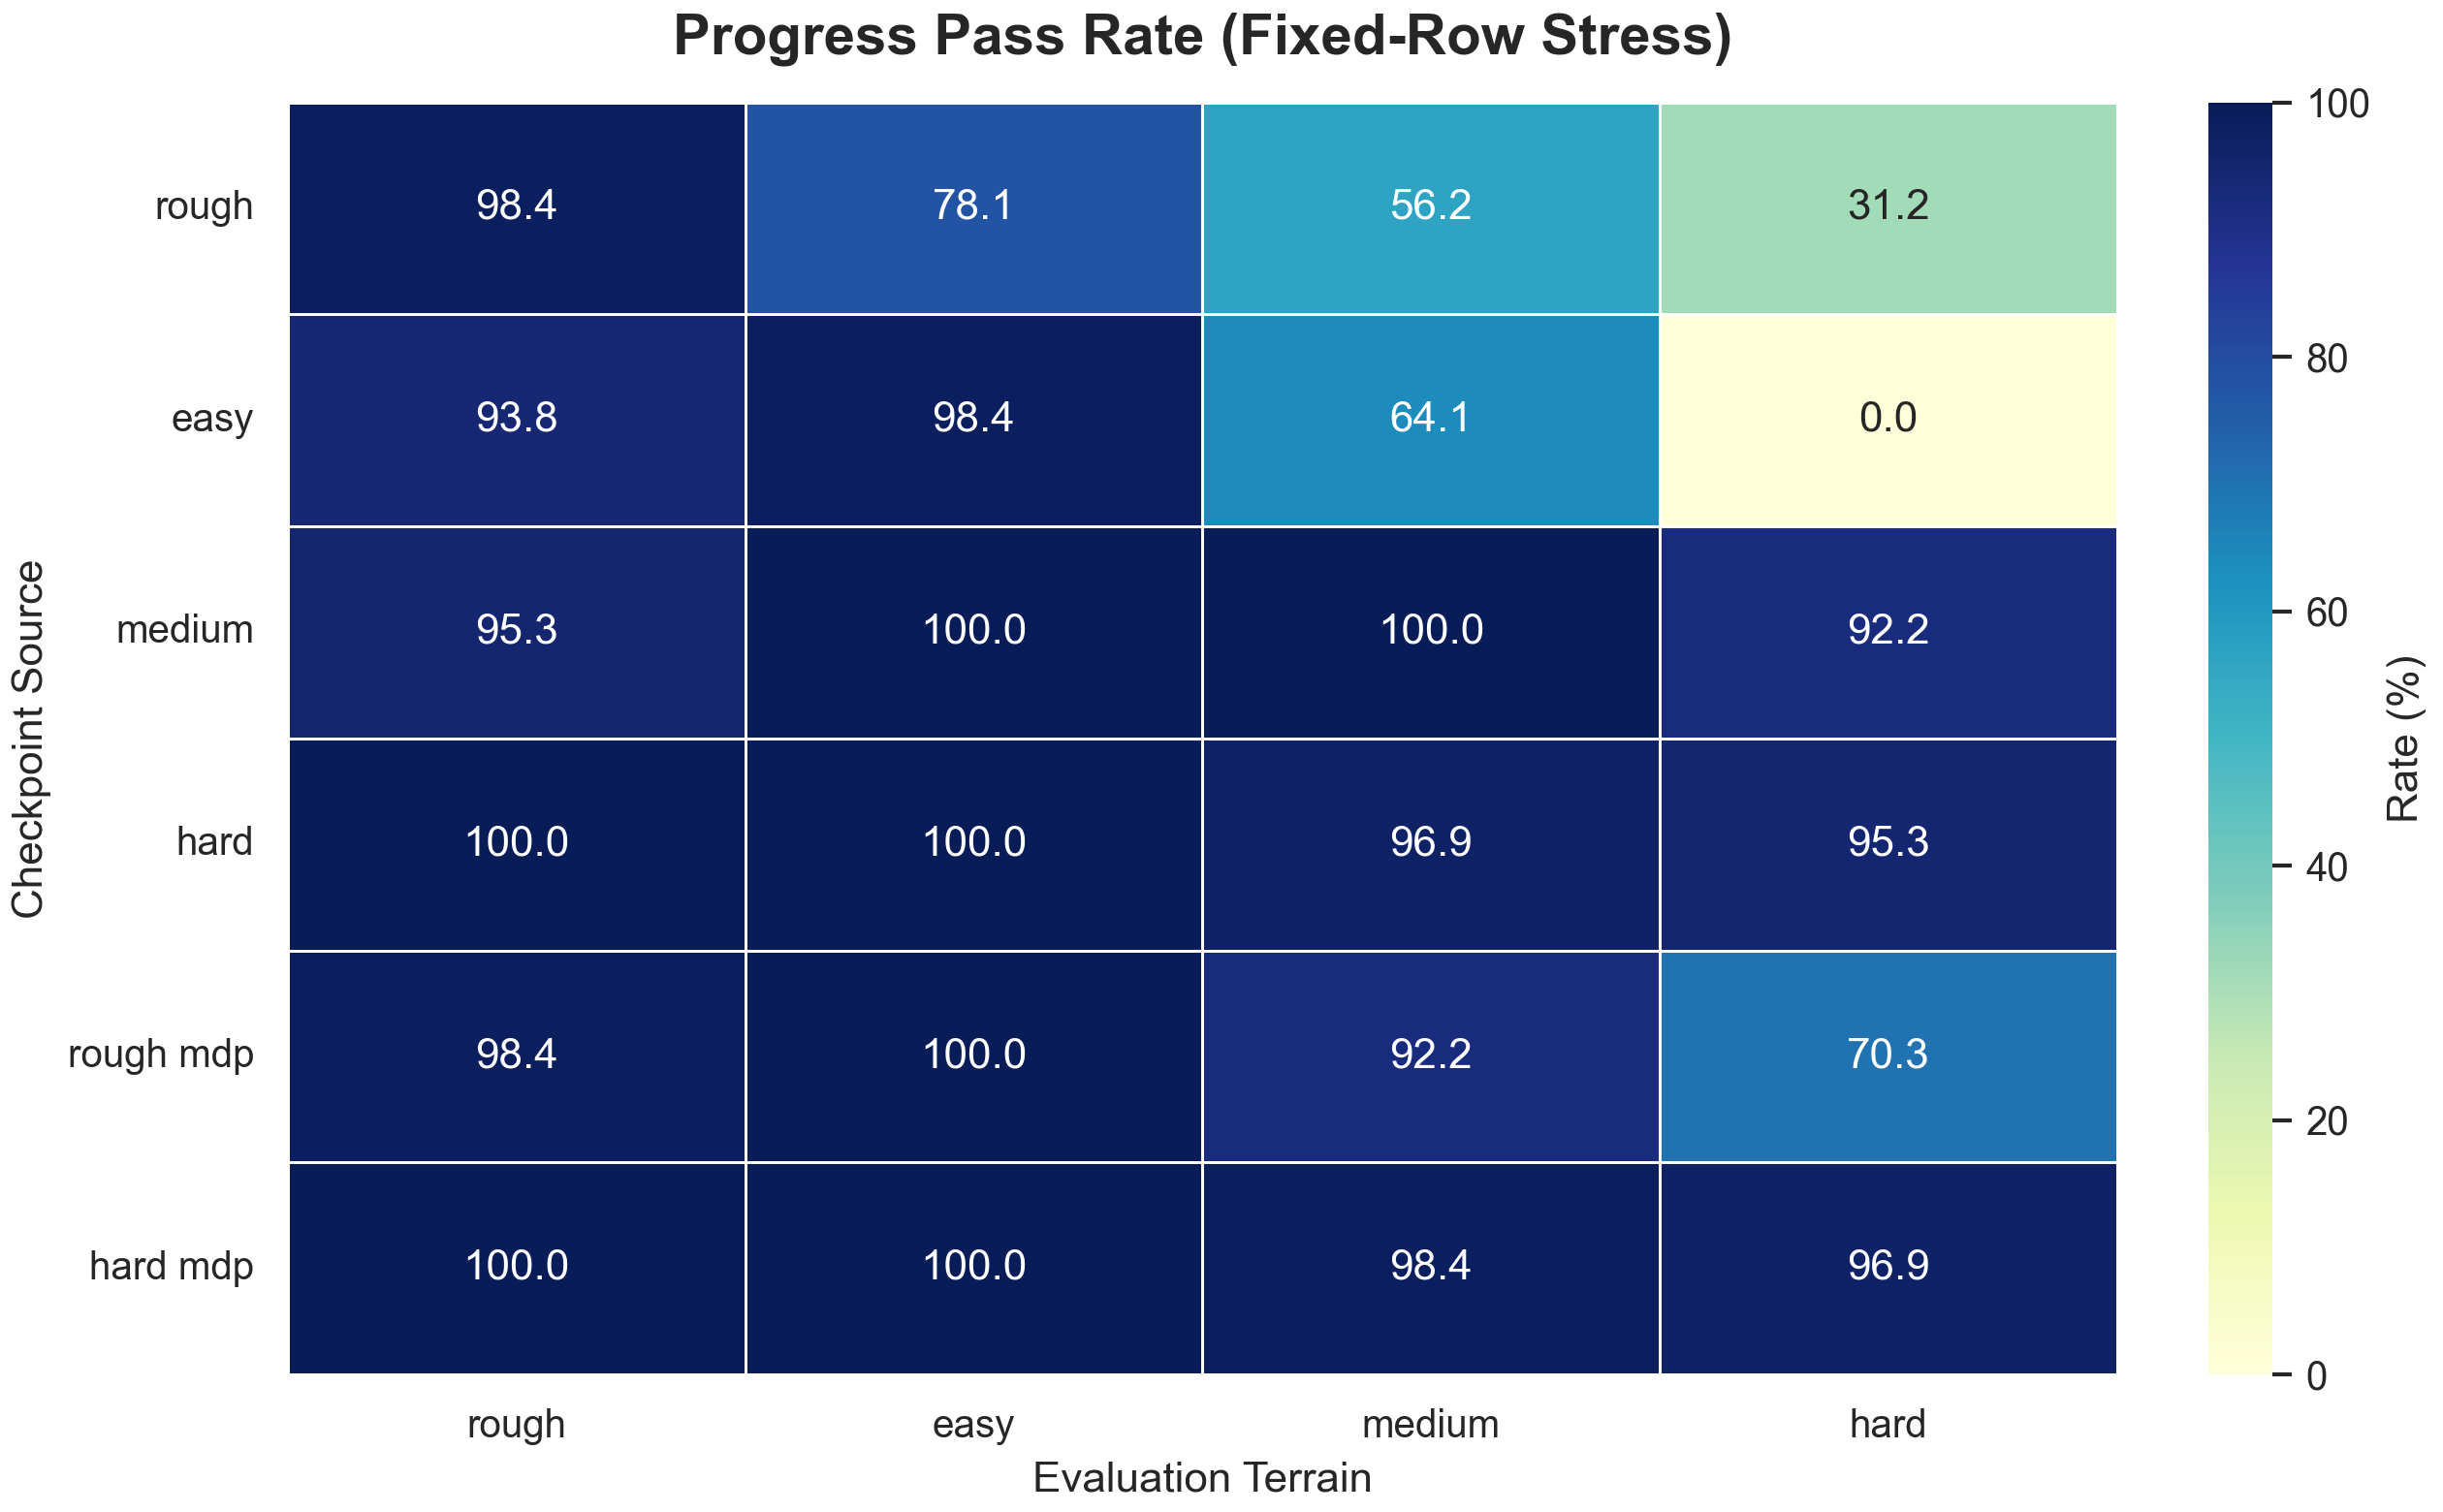
\includegraphics[width=\linewidth]{figures/progress_stress_heatmap.png}
        \caption{Progress}
    \end{subfigure}
    \hfill
    \begin{subfigure}[t]{0.32\linewidth}
        \centering
        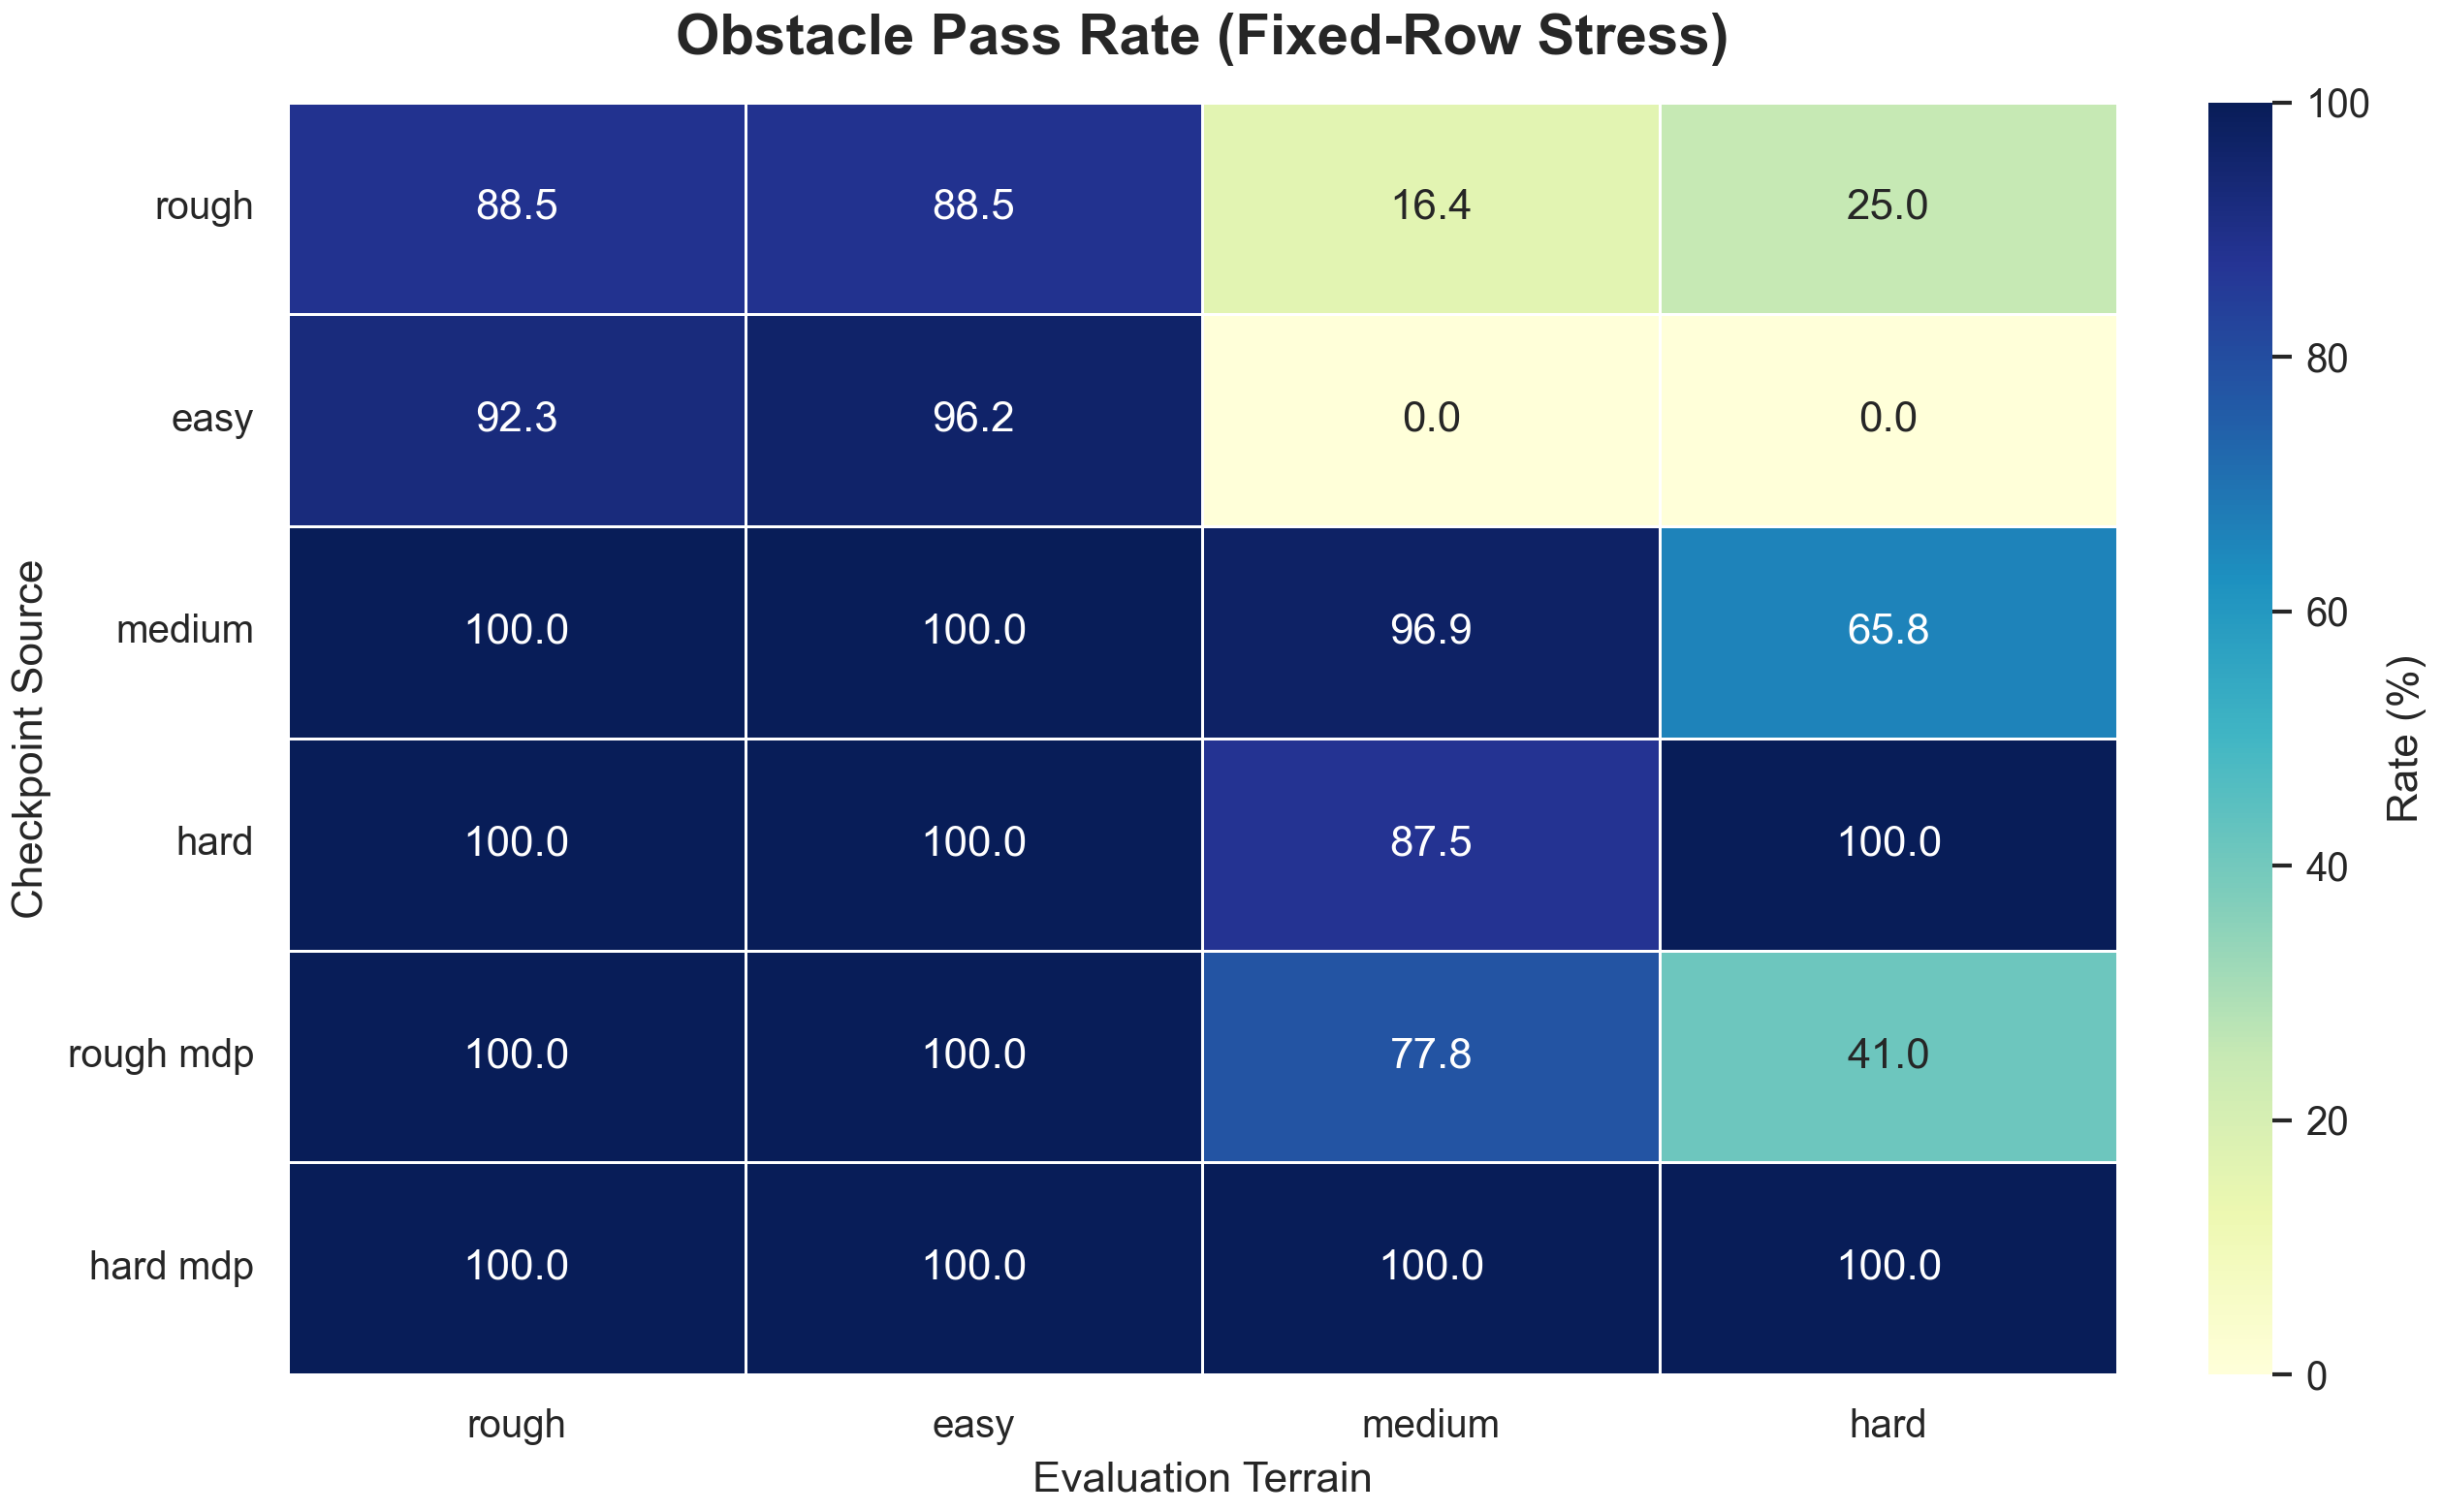
\includegraphics[width=\linewidth]{figures/obstacle_stress_heatmap.png}
        \caption{Obstacle}
    \end{subfigure}
    \caption{\textbf{Stress cross-terrain heatmaps.} Survival and progress show similar transfer patterns, while obstacle crossing exposes terrain-specific failures that timeout alone can hide.}
    \label{fig:stress-heatmaps}
\end{figure}

\Cref{fig:stress-heatmaps} summarizes the fixed-row stress protocol. The heatmaps make the main pattern visible: rough and easy policies do not transfer reliably to medium or hard obstacles, medium training is the first setting with strong hard-terrain survival, and hard training gives the most consistent source policy.

\subsubsection{Timeout}

\begin{table}[t]
    \caption{\textbf{Random cross-terrain timeout rate.}}
    \label{tab:random-cross-timeout}
    \centering
    \begin{tabular}{lcccc}
        \toprule
        Source & Eval rough & Eval easy & Eval medium & Eval hard \\
        \midrule
        Rough & 95.31\% & 98.44\% & 68.75\% & 29.69\% \\
        Easy & 90.62\% & 100.00\% & 50.00\% & 0.00\% \\
        Medium & 98.44\% & 98.44\% & 95.31\% & 87.50\% \\
        Hard & 100.00\% & 100.00\% & 96.88\% & 95.31\% \\
        \bottomrule
    \end{tabular}
\end{table}

\begin{table}[t]
    \caption{\textbf{Stress cross-terrain timeout rate.}}
    \label{tab:stress-cross-timeout}
    \centering
    \begin{tabular}{lcccc}
        \toprule
        Source & Eval rough & Eval easy & Eval medium & Eval hard \\
        \midrule
        Rough & 98.44\% & 78.12\% & 56.25\% & 31.25\% \\
        Easy & 95.31\% & 98.44\% & 50.00\% & 0.00\% \\
        Medium & 95.31\% & 100.00\% & 95.31\% & 92.19\% \\
        Hard & 100.00\% & 100.00\% & 96.88\% & 95.31\% \\
        \bottomrule
    \end{tabular}
\end{table}

\Cref{tab:random-cross-timeout} shows the random timeout evaluation results. The rough and easy checkpoints perform poorly on the medium and hard environments, while the medium and hard checkpoints remain strong across all evaluation environments. Among them, the hard checkpoint has the best overall generalization ability. \Cref{tab:stress-cross-timeout} reports the timeout results under the fixed-row stress protocol. The overall trend is consistent with the random evaluation, but rough-to-easy and rough-to-medium performance drops noticeably under stress, which is likely caused by the increased terrain difficulty in the stress setting.

\subsubsection{Traversal progress}

\begin{table}[t]
    \caption{\textbf{Random cross-terrain traversal progress rate.}}
    \label{tab:random-cross-progress}
    \centering
    \begin{tabular}{lcccc}
        \toprule
        Source & Eval rough & Eval easy & Eval medium & Eval hard \\
        \midrule
        Rough & 95.31\% & 98.44\% & 68.75\% & 29.69\% \\
        Easy & 89.06\% & 100.00\% & 50.00\% & 0.00\% \\
        Medium & 98.44\% & 98.44\% & 95.31\% & 87.50\% \\
        Hard & 100.00\% & 100.00\% & 96.88\% & 95.31\% \\
        \bottomrule
    \end{tabular}
\end{table}

\begin{table}[t]
    \caption{\textbf{Stress cross-terrain traversal progress rate.}}
    \label{tab:stress-cross-progress}
    \centering
    \begin{tabular}{lcccc}
        \toprule
        Source & Eval rough & Eval easy & Eval medium & Eval hard \\
        \midrule
        Rough & 98.44\% & 78.12\% & 56.25\% & 31.25\% \\
        Easy & 93.75\% & 98.44\% & 64.06\% & 0.00\% \\
        Medium & 95.31\% & 100.00\% & 100.00\% & 92.19\% \\
        Hard & 100.00\% & 100.00\% & 98.44\% & 96.88\% \\
        \bottomrule
    \end{tabular}
\end{table}


\Cref{tab:random-cross-progress,tab:stress-cross-progress} show the random and stress traversal-progress results respectively. The progress results are almost identical to the timeout results, with the largest difference being only 1.56 percentage points. This indicates that once the robot avoids falling, it almost always continues moving in the correct forward direction. Therefore, timeout and traversal progress produce nearly the same evaluation pattern.

\subsubsection{Obstacle crossing}

\begin{table}[t]
    \caption{\textbf{Stress cross-terrain obstacle crossing rate.} Hard training gives the strongest overall source policy.}
    \label{tab:stress-cross-obstacle}
    \centering
    \begin{tabular}{lcccc}
        \toprule
        Source & Eval rough & Eval easy & Eval medium & Eval hard \\
        \midrule
        Rough & 88.46\% & 88.46\% & 16.39\% & 25.00\% \\
        Easy & 92.31\% & 96.15\% & 0.00\% & 0.00\% \\
        Medium & 100.00\% & 100.00\% & 96.88\% & 65.79\% \\
        Hard & 100.00\% & 100.00\% & 87.50\% & 100.00\% \\
        \bottomrule
    \end{tabular}
\end{table}

To improve the determinism of obstacle-crossing evaluation, I use only the fixed-row stress protocol for this metric. \Cref{tab:stress-cross-obstacle} reports the stress obstacle-crossing results. The overall trend is still consistent with the stress timeout results, but the obstacle-crossing success rates drop substantially for rough and easy on the medium and hard environments, and also for medium on the hard environment. This shows that avoiding falls does not necessarily mean that the robot has successfully crossed complex obstacles such as stairs and gaps. The hard checkpoint again shows the strongest overall performance in this evaluation.

\section{Ablation experiments}
\label{sec:ablations}

\subsection{MDP ablation}
The MDP ablation evaluates whether lightweight reward shaping can improve obstacle competence without changing the robot, action space, observation space, terrain generator, or training budget. Two variants are trained: \texttt{rough\_mdp} on official rough terrain and \texttt{hard\_mdp} on hard parkour terrain.

\begin{figure}[t]
    \centering
    \begin{subfigure}[t]{0.48\linewidth}
        \centering
        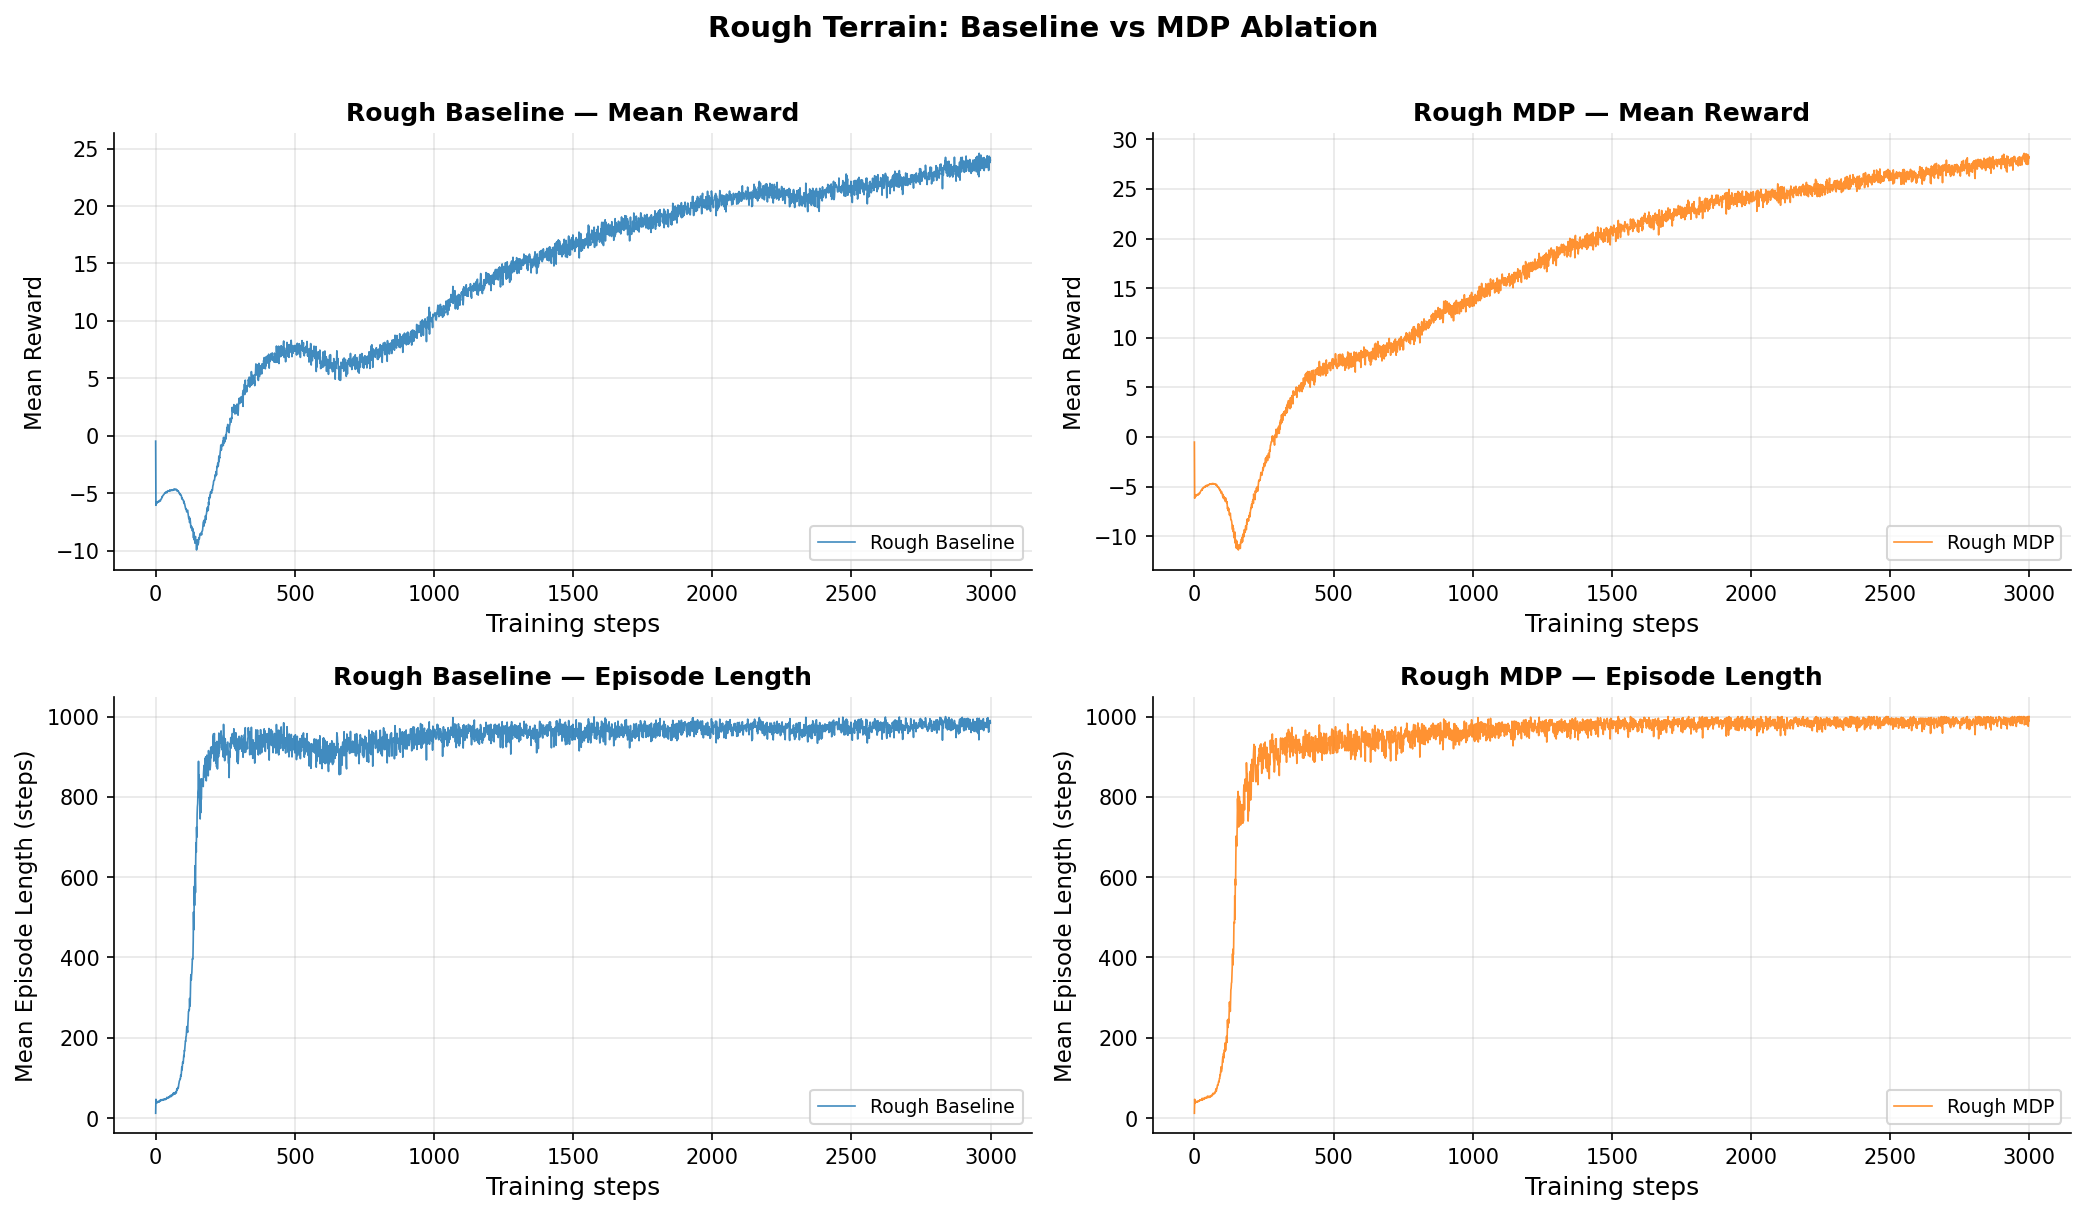
\includegraphics[width=\linewidth]{figures/mdp_ablation_rough_comparison.png}
        \caption{Rough vs. Rough MDP}
    \end{subfigure}
    \hfill
    \begin{subfigure}[t]{0.48\linewidth}
        \centering
        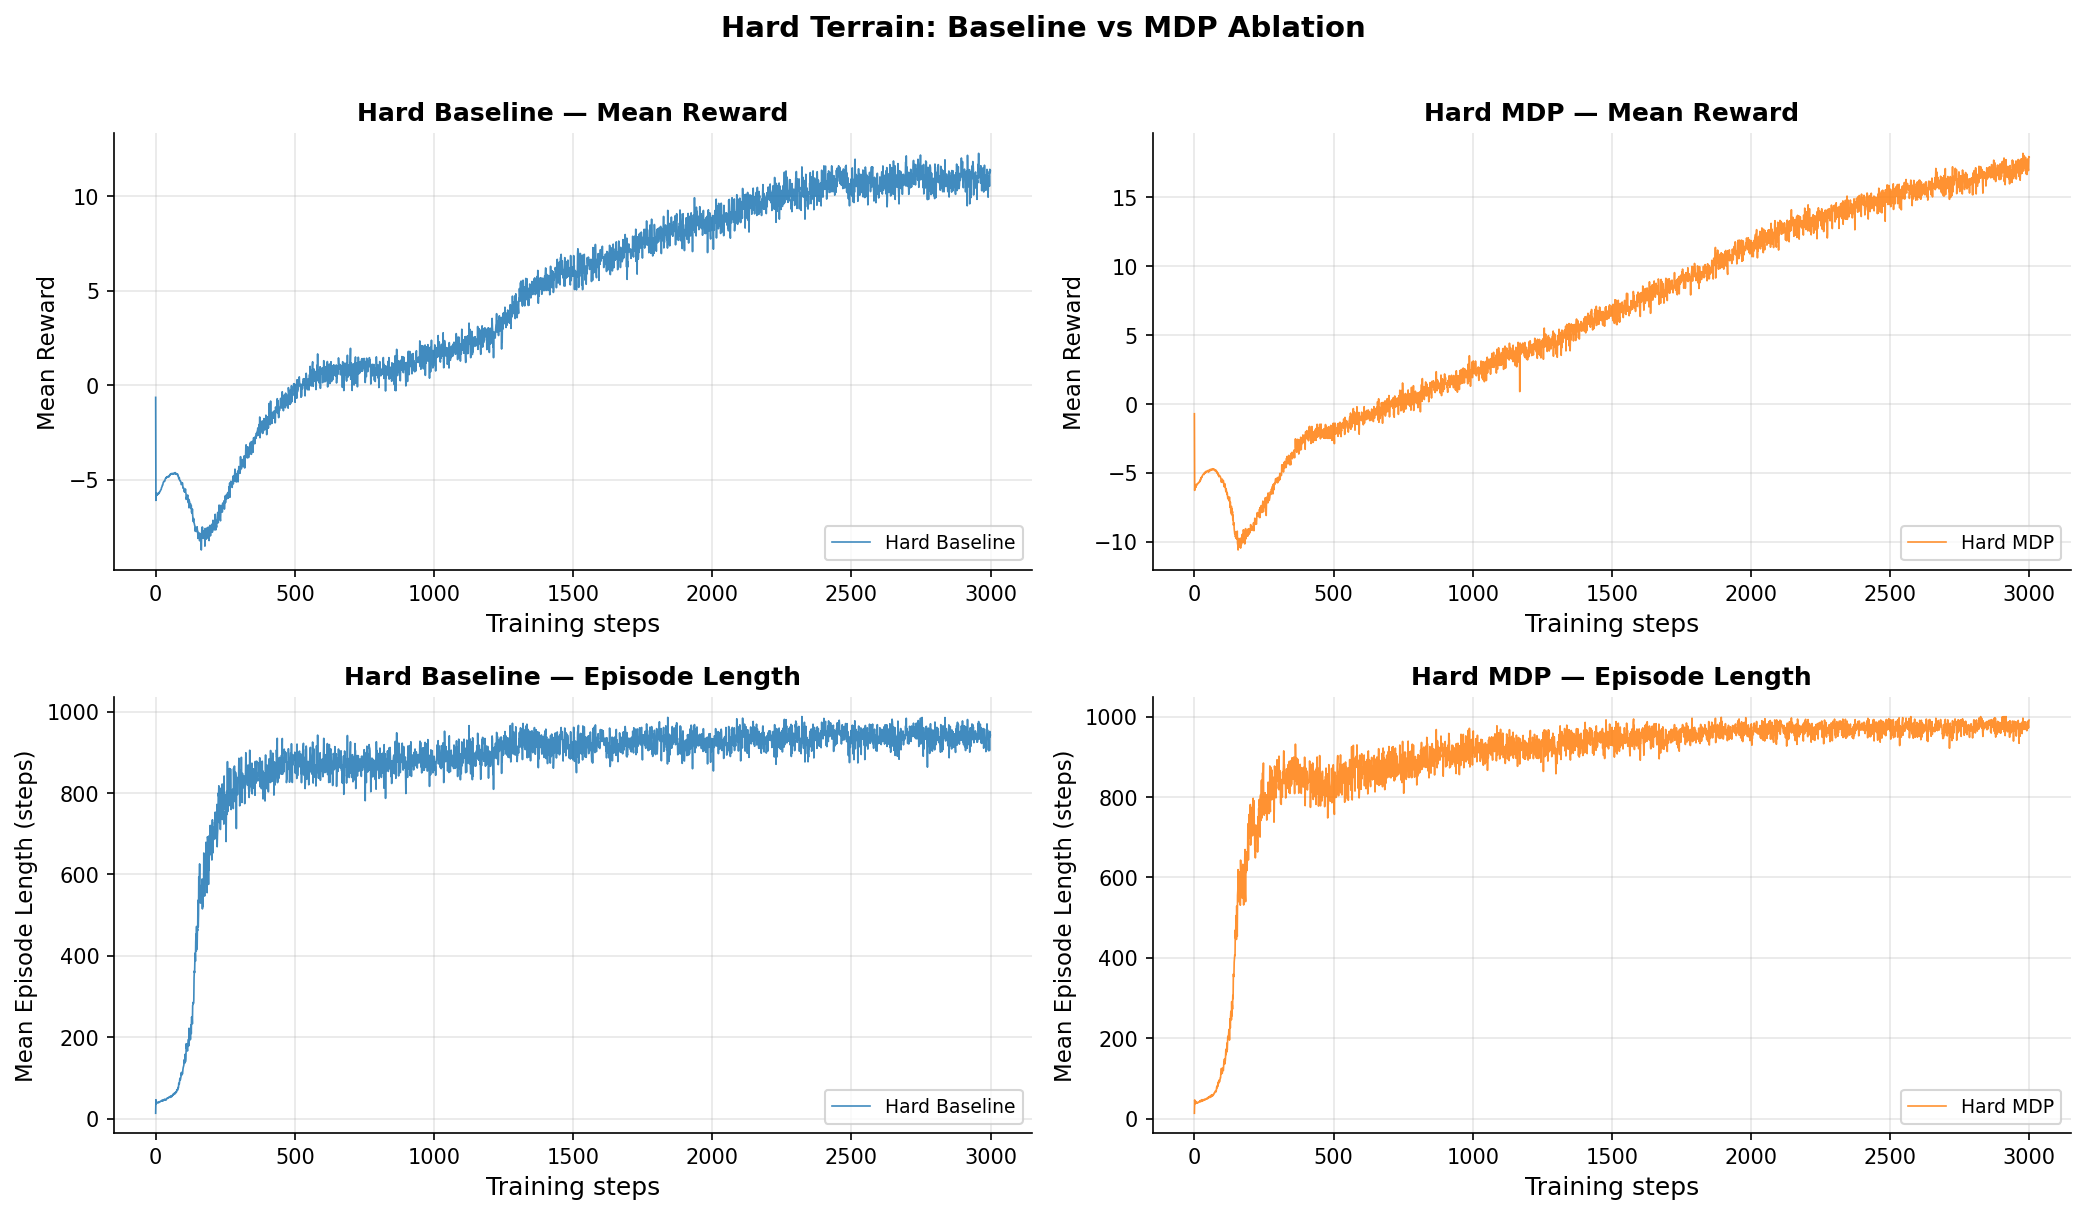
\includegraphics[width=\linewidth]{figures/mdp_ablation_hard_comparison.png}
        \caption{Hard vs. Hard MDP}
    \end{subfigure}
    \caption{\textbf{MDP ablation training comparison.} Reward shaping improves episode stability and final training statistics, but the policy comparison is interpreted using the shared evaluation metrics below because reward scales differ across MDPs.}
    \label{fig:mdp-ablation-training}
\end{figure}

\begin{table}[t]
    \caption{\textbf{Final training summary for MDP ablation.} Rough and hard baselines are compared with their corresponding reward-shaped MDP variants under the same 3000-iteration budget.}
    \label{tab:mdp-training}
    \centering
    \begin{tabular}{lcccc}
        \toprule
        Metric & Rough & Rough MDP & Hard & Hard MDP \\
        \midrule
        Mean reward & 24.01 & 28.25 & 11.34 & 17.93 \\
        Mean episode length & 984.5 & 1000.0 & 941.7 & 991.2 \\
        Timeout rate & 94.62\% & 97.85\% & 89.08\% & 95.29\% \\
        Fall rate & 5.41\% & 2.15\% & 10.92\% & 4.71\% \\
        XY tracking error & 0.3407 & 0.3718 & 0.4407 & 0.4274 \\
        Yaw tracking error & 0.7501 & 0.6676 & 1.0088 & 0.9165 \\
        Curriculum level & 5.7961 & 5.705 & 5.6389 & 5.769 \\
        \bottomrule
    \end{tabular}
\end{table}

\begin{table}[t]
    \caption{\textbf{MDP ablation obstacle-crossing comparison.} Obstacle crossing is evaluated under the fixed-row stress protocol and only includes supported gap and stairs terrain groups.}
    \label{tab:mdp-obstacle}
    \centering
    \begin{tabular}{lcccc}
        \toprule
        Source & Eval rough & Eval easy & Eval medium & Eval hard \\
        \midrule
        Rough & 88.46\% & 88.46\% & 16.39\% & 25.00\% \\
        Rough MDP & 100.00\% & 100.00\% & 77.78\% & 41.03\% \\
        Hard & 100.00\% & 100.00\% & 87.50\% & 100.00\% \\
        Hard MDP & 100.00\% & 100.00\% & 100.00\% & 100.00\% \\
        \bottomrule
    \end{tabular}
\end{table}

\Cref{fig:mdp-ablation-training,tab:mdp-training} show the training results after modifying the MDP. Most training metrics improve noticeably, especially episode length and fall rate. However, because the reward definition is different, the training reward should not be used as the sole evidence that the new policy is stronger. A fair comparison still requires evaluating the policies under the same timeout, progress, and obstacle metrics.

\Cref{tab:mdp-obstacle} reports the fixed-row stress obstacle-crossing results for the MDP-shaped policies. Since parkour ability is the main focus, timeout and traversal-progress results are not repeated here. The results show clear improvements for both Rough MDP and Hard MDP. In particular, Rough MDP improves obstacle-crossing success on the medium environment by 61.39 percentage points over the rough baseline. This suggests that the modified MDP, namely the added \texttt{parkour\_progress} and \texttt{foothold\_safety} rewards, substantially improves the policy's obstacle-crossing ability. It also indicates that a moderately more conservative behavior pattern can have a positive effect on learning to cross obstacles.

\subsection{ExtremeRandom OOD stress}

Since both Hard and Hard MDP achieve near-perfect performance in the standard obstacle-crossing evaluation, this metric does not clearly distinguish their capabilities. Therefore, I introduce an ExtremeRandom environment that is harder than the hard obstacle environment, and compare Hard and Hard MDP under this more challenging setting. \Cref{fig:extreme} shows the evaluation results. Hard MDP achieves a clear advantage over Hard: the overall obstacle pass rate improves by 29.8 percentage points, gap pass rate improves by 5.5 percentage points, and stairs pass rate improves by a much larger 54.3 percentage points. These results indicate that the modified MDP also provides a substantial improvement for the hard policy.

\begin{figure}[t]
    \centering
    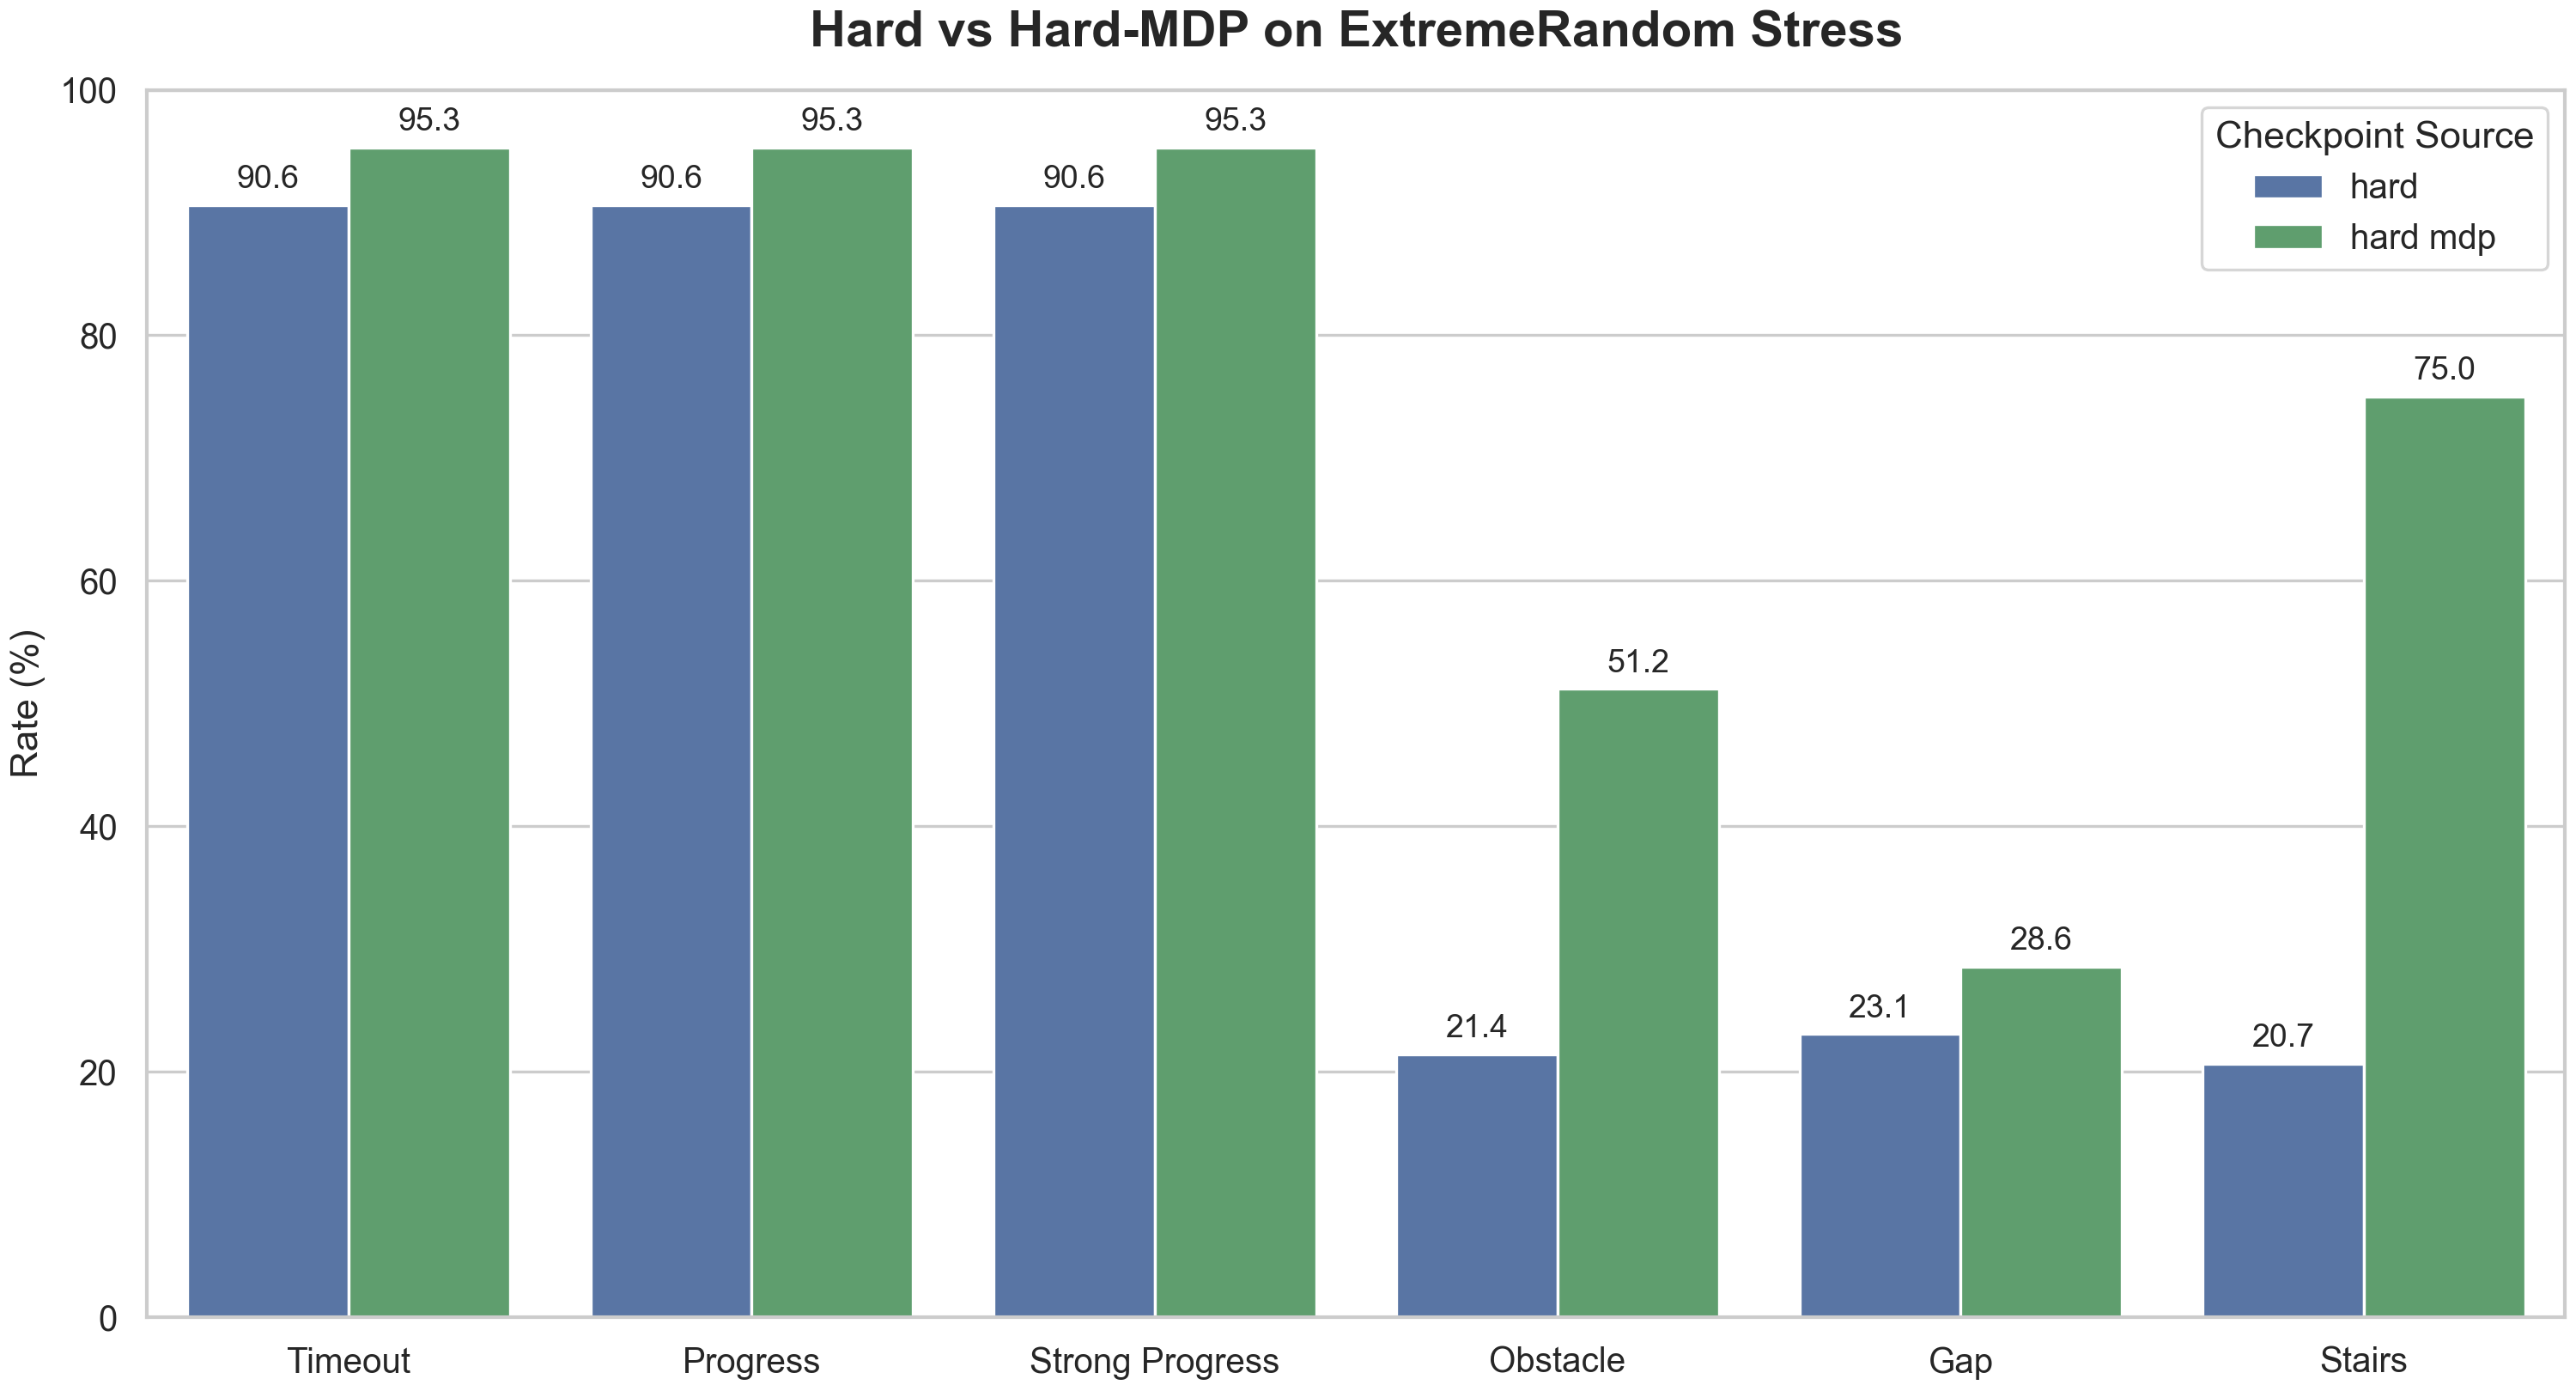
\includegraphics[width=0.72\linewidth]{figures/extreme_hard_vs_hard_mdp_bar.png}
    \caption{\textbf{ExtremeRandom hard vs. hard-MDP comparison.} Hard MDP improves survival and obstacle crossing on a harsher evaluation-only terrain distribution.}
    \label{fig:extreme}
\end{figure}

\section{Discussion}
\label{sec:discussion}

The results establish a progression from flat locomotion to rough locomotion and then to structured parkour. Flat terrain is nearly solved. Rough terrain increases failure and tracking error but remains trainable. Easy parkour is stable but narrow: it performs well on its own terrain but fails to transfer to hard. Medium parkour is the minimum completed terrain tier with strong hard-terrain survival transfer, but obstacle crossing reveals that medium still lacks reliable hard-gap competence. Hard parkour is the strongest source policy and fully solves the supported hard gap and stairs boundaries under stress.

The MDP ablation shows that reward design is not only a fine-tuning detail. Rough MDP substantially improves hard-terrain transfer without parkour terrain exposure, suggesting that the inherited velocity-tracking reward alone underuses available terrain information. On hard terrain, the additional foothold-safety cost makes the policy more conservative. This reduces average forward distance but improves tracking precision and out-of-distribution obstacle crossing. For parkour locomotion, this tradeoff is acceptable because carefully crossing obstacles is more important than maximizing raw forward speed.

The main limitation is metric semantics. Timeout measures survival, traversal progress checks forward movement, and obstacle crossing checks base-level boundary completion. These are sufficient for the current terrain generator, but they do not directly measure foot-contact quality, exact foothold placement, or mesh-level contact safety. Future work should therefore add stricter contact-aware metrics, broader out-of-distribution obstacle layouts, and optionally motion-prior methods such as AMP/SMP-style regularization.

\section{Conclusion}
\label{sec:conclusion}

This project implements a complete custom parkour locomotion pipeline for Unitree G1 in Isaac Lab. It defines three increasing terrain tiers, trains PPO policies for each tier, evaluates cross-terrain generalization with three metric families, and studies reward-shaping effects through MDP ablations. The main empirical findings are:
\begin{itemize}[leftmargin=*,noitemsep,nolistsep,topsep=0pt]
    \item terrain difficulty increases clearly from easy to medium to hard in reward, fall rate, and tracking error;
    \item medium is the first tier with strong survival transfer to hard terrain, but hard-gap crossing remains limited;
    \item hard training gives the best overall source checkpoint, reaching at least 95.31\% timeout rate across evaluation environments and 100.00\% hard gap/stairs obstacle pass under stress;
    \item MDP reward shaping improves rough-to-hard timeout from 29.69\% to 70.31\% without parkour terrain exposure;
    \item Hard MDP improves precision and ExtremeRandom obstacle crossing while adopting a more conservative forward-speed profile.
\end{itemize}
Together, these results support the feasibility of using Isaac Lab's G1 rough locomotion stack as a base for structured humanoid parkour and provide a reproducible foundation for further navigation-style or foothold-aware extensions.

\end{document}
